\documentclass[12pt]{article}
\usepackage[utf8]{inputenc}
\usepackage[margin=1in]{geometry}
\usepackage{caption} % figure captioning
\usepackage{amsmath} % equation tools
\usepackage{amssymb} % math symbols
\usepackage{mathtools} % math rendering improvements
\usepackage{siunitx} % standard units
\usepackage{graphicx} % add images
%\usepackage{wrapfig} % position images
\usepackage{float} % position images pt.2
%\usepackage[makeroom]{cancel} % cross out text
%\usepackage[version=4]{mhchem} % chemical equations
%\usepackage{multicol} % multiple columns
%\usepackage{pgfplots} % built in plotter
%\pgfplotsset{width=10cm,compat=1.9} % plotter settings

\renewcommand{\baselinestretch}{1.5} % line spacing
\newcommand{\fline}{\par\noindent\rule{\textwidth}{0.1pt}} % horizontal line (wide)

\sisetup{per-mode=fraction}

\title{Factors Affecting Resistance Lab Report}
\author{Bryan Deng}

\begin{document}

\maketitle
\newpage
\tableofcontents
\newpage

\section{Design}

\subsection{Materials}

\begin{itemize}
    \item paper
    \item graphite pencil
    \item multimeter
    \item ruler
\end{itemize}

\subsection{Purpose}

To determine how length and width (cross-sectional area) affect the resistance of a "wire".

\subsection{Procedure}

\begin{enumerate}
    \item Using the ruler and pencil, draw out 4 lines of the following dimensions:
    \begin{enumerate}
        \item length: $5\si{cm} \pm 0.05\si{cm}$, width: $0.5\si{cm} \pm 0.05\si{cm}$
        \item length: $5\si{cm} \pm 0.05\si{cm}$, width: $2\si{cm} \pm 0.05\si{cm}$
        \item length: $10\si{cm} \pm 0.05\si{cm}$, width: $0.5\si{cm} \pm 0.05\si{cm}$
        \item length: $10\si{cm} \pm 0.05\si{cm}$, width: $2\si{cm} \pm 0.05\si{cm}$
    \end{enumerate}
    \item Ensure that each line is completely and thoroughly filled in with graphite.
    \item For each line, measure the resistance by putting the tips of the multimeter on opposite ends, along the length of the line.
    \item Record data for each line in a table.
\end{enumerate}

\subsection{Diagrams}

\begin{figure}[H]
    \centering
    \fbox{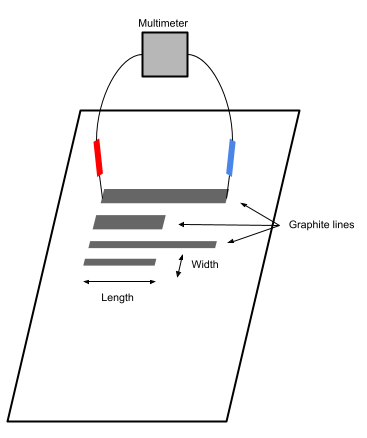
\includegraphics[scale=0.7]{images/setup.png}}
    \caption{Diagram of lines and multimeter setup}
    \label{fig:diagram}
\end{figure}

\section{Qualitative Observations}

\begin{itemize}
    \item The ends of the multimeter were not held completely still during each trial, so there was a constant fluctuation in the resistance readings.
\end{itemize}

\newpage

\section{Data Tables}

\begin{center}
    \captionof{table}{How width affects resistance, measured on $5\si{cm}$ long line}
    \begin{tabular}{|c|c|}
        \hline
        \textbf{Width} & \textbf{Resistance} \\
        \hline \hline
        $0.5\si{cm} \pm 0.05\si{cm}$ & $0.280\si{\mega\ohm} \pm 0.005\si{\mega\ohm}$ \\
        \hline
        $2\si{cm} \pm 0.05\si{cm}$ & $0.032\si{\mega\ohm} \pm 0.005\si{\mega\ohm}$ \\
        \hline
    \end{tabular}
\end{center}

\begin{center}
    \captionof{table}{How length affects resistance, measured on $0.5\si{cm}$ wide line}
    \begin{tabular}{|c|c|}
        \hline
        \textbf{Length} & \textbf{Resistance} \\
        \hline \hline
        $5\si{cm} \pm 0.05\si{cm}$ & $0.280\si{\mega\ohm} \pm 0.005\si{\mega\ohm}$ \\
        \hline
        $10\si{cm} \pm 0.05\si{cm}$ & $0.303\si{\mega\ohm} \pm 0.005\si{\mega\ohm}$ \\
        \hline
    \end{tabular}
\end{center}

\begin{center}
    \captionof{table}{Calculated slopes between factors that affect resistance and resistance}
    \begin{tabular}{|c|c|}
        \hline
        \textbf{Variable} & \textbf{Calculated Value} \\
        \hline \hline
        Slope of resistance over width & $m_w = (-0.17 \pm 0.02) \si{\mega\ohm\per\cm}$ \\
        \hline
        Slope of resistance over length & $m_l = (0.005 \pm 0.002) \si{\mega\ohm\per\cm}$ \\
        \hline
    \end{tabular}
\end{center}

\section{Plots}

\begin{figure}[H]
    \centering
    \fbox{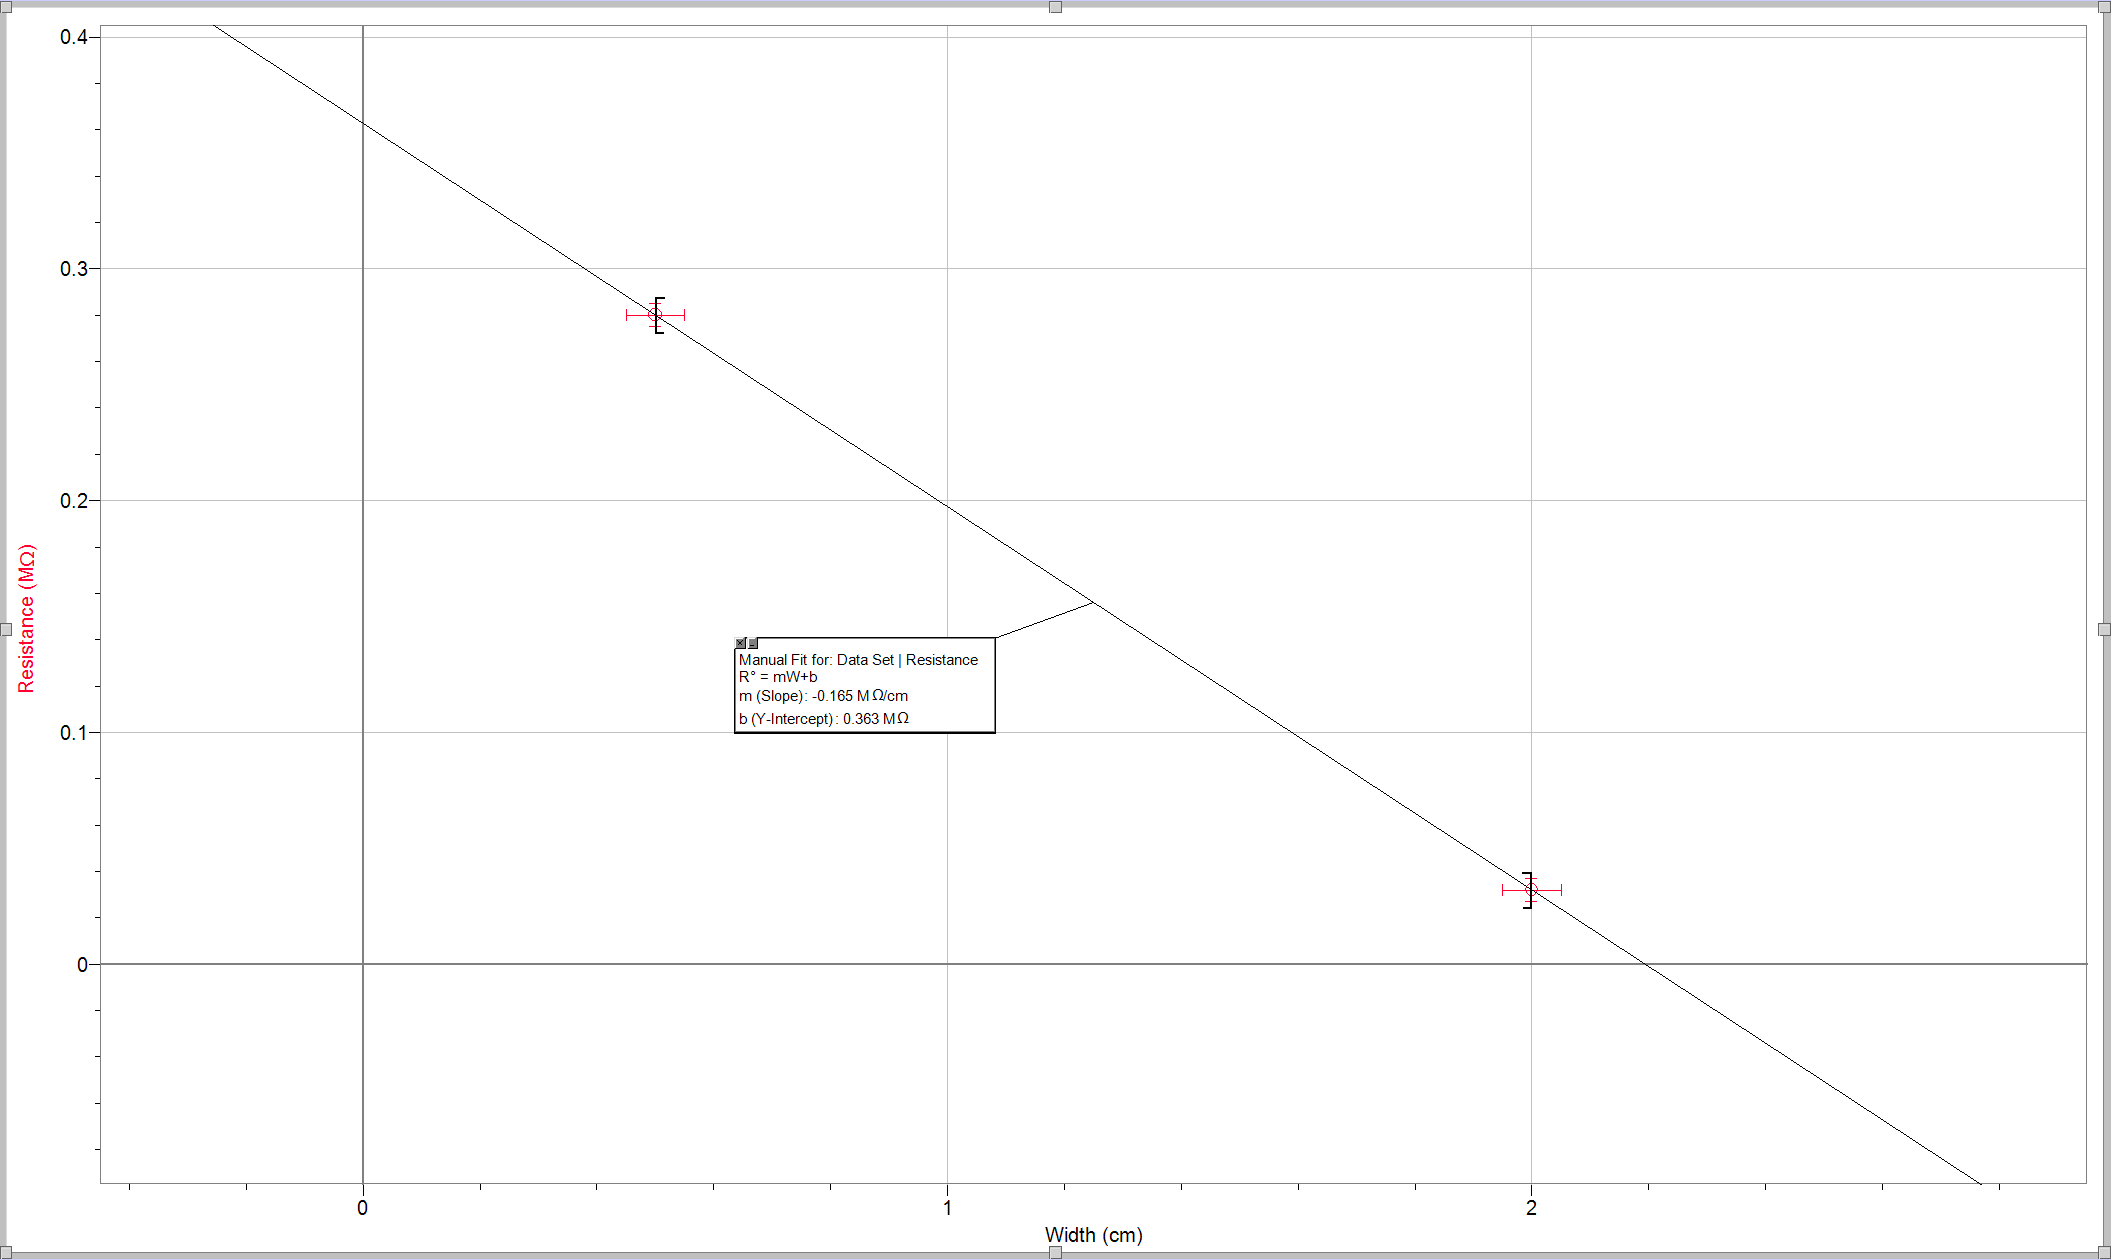
\includegraphics[scale=0.3]{images/plot_width2.png}}
    \caption{How width affects resistance, measured on $5\si{cm} \pm 0.05\si{cm}$ long line}
    \label{plot:width}
\end{figure}

\begin{figure}[H]
    \centering
    \fbox{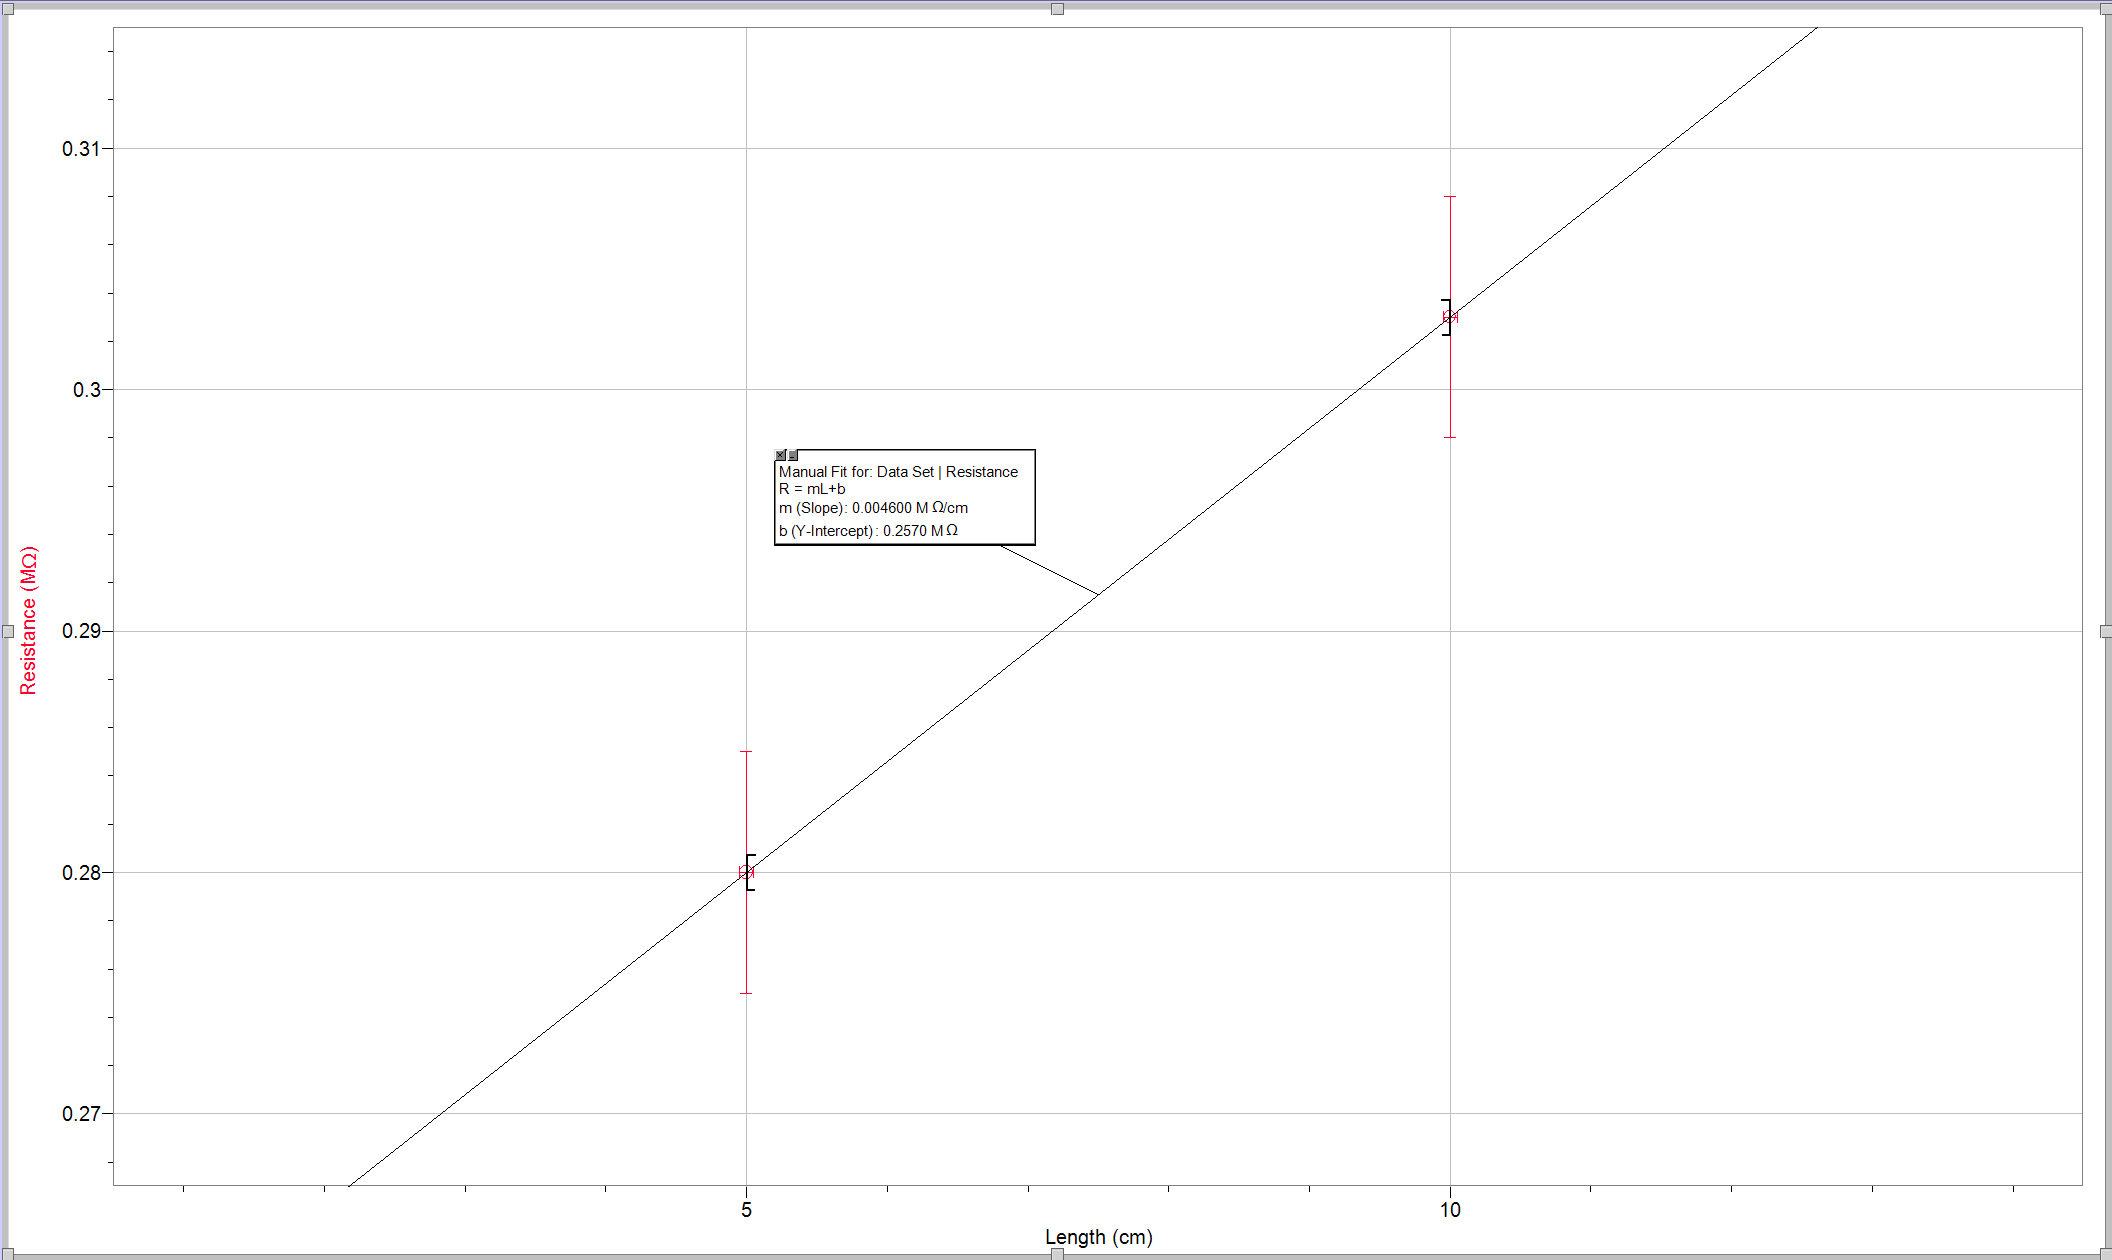
\includegraphics[scale=0.3]{images/plot_length2.png}}
    \caption{How length affects resistance, measured on $0.5\si{cm} \pm 0.05\si{cm}$ wide line}
    \label{plot:length}
\end{figure}

\section{Analysis}

\subsection{Slope of Resistance Over Width}

\begin{align*}
    m_w &= \frac{\Delta y}{\Delta x} \\[10pt]
    &= \frac{y_1 - y_2}{x_1 - x_2} \\[10pt]
    &= \frac{(0.280 \pm 0.005)\si{\mega\ohm} - (0.032 \pm 0.005)\si{\mega\ohm}}{(0.5 \pm 0.05)\si{cm} - (2 \pm 0.05)\si{cm}} \\[10pt]
    &= \frac{(0.280 - 0.032)\si{\mega\ohm} \pm (0.005 + 0.005)\si{\mega\ohm}}{(0.5 - 2)\si{cm} \pm (0.05 - 0.05)\si{cm}} \\[10pt]
    &= \frac{(0.248 \pm 0.01)\si{\mega\ohm}}{(-1.5 \pm 0.1)\si{cm}} \\[10pt]
    &= \left( \left( \frac{0.248}{-1.5} \right) \pm \left( \left| \frac{0.01}{0.248} \right| + \left| \frac{0.1}{-1.5} \right| \right) \times 100\% \right) \si{\mega\ohm\per\cm} \\[10pt]
    &= (-0.165 \pm 10.699\%) \si{\mega\ohm\per\cm} \\
    \Aboxed{m_w &= (-0.17 \pm 0.02) \si{\mega\ohm\per\cm}}
\end{align*}

\subsection{Slope of Resistance Over Length}

\begin{align*}
    m_l &= \frac{\Delta y}{\Delta x} \\[10pt]
    &= \frac{y_1 - y_2}{x_1 - x_2} \\[10pt]
    &= \frac{(0.280 \pm 0.005)\si{\mega\ohm} - (0.303 \pm 0.005)\si{\mega\ohm}}{(5 \pm 0.05)\si{cm} - (10 \pm 0.05)\si{cm}} \\[10pt]
    &= \frac{(0.280 - 0.303)\si{\mega\ohm} \pm (0.005 + 0.005)\si{\mega\ohm}}{(5 - 10)\si{cm} \pm (0.05 - 0.05)\si{cm}} \\[10pt]
    &= \frac{(-0.023 \pm 0.01)\si{\mega\ohm}}{(-5 \pm 0.1)\si{cm}} \\[10pt]
    &= \left( \left( \frac{-0.023}{-5} \right) \pm \left( \left| \frac{0.01}{-0.023} \right| + \left| \frac{0.1}{-5} \right| \right) \times 100\% \right) \si{\mega\ohm\per\cm} \\[10pt]
    &= (0.005 \pm 45.478\%) \si{\mega\ohm\per\cm} \\
    \Aboxed{m_l &= (0.005 \pm 0.002) \si{\mega\ohm\per\cm}}
\end{align*}

\newpage

\section{Error Discussion}

\subsection{Random Errors}

\begin{itemize}
    \item It is impossible to completely fill in the lines with graphite, or maintain a consistent density of shading throughout the line, or across different lines. Therefore the resistance may fluctuate throughout the length of the line.
\end{itemize}

\subsection{Methodological Errors}

\begin{itemize}
    \item Given the short time constraint, it was not possible to conduct further trials and generate a larger dataset. The smaller dataset is more prone to errors.
    \begin{itemize}
        \item It is impossible to determine whether the relationship between each factor and resistance is linear or non-linear as there are only 2 data points per factor.
    \end{itemize}
    \item Furthermore, only a single trial was conducted for each line. Although the measurements are accounted for by uncertainties, the entire dataset depends on this single trial. Therefore, if this one trial was off, it would not be possible to correct it by averaging it out with other values.
\end{itemize}

\section{Conclusion}

\subsection{Width (Cross-sectional Area)}

Based on the conclusion that the change in resistance over change in width is:
\begin{gather*}
    m_w = (-0.17 \pm 0.02) \si{\mega\ohm\per\cm}.
\end{gather*}
Resistance is negatively proportional to width, as $m_w < 0$. For every $1\si{cm}$ that width increases, resistance decreases by $(-0.17 \pm 0.02)\si{\mega\ohm}$. Furthermore, because the experiment is based on a 2 dimensional plane, the width of the graphite line is equivalent to cross sectional area ($A$) in the third dimension. Therefore the experimental conclusion is:
\begin{gather*}
    R \propto -A
\end{gather*}

\subsection{Length}

Based on the conclusion that the change in resistance over the change in length is:
\begin{gather*}
    m_l = (0.005 \pm 0.002) \si{\mega\ohm\per\cm}.
\end{gather*}
Resistance is directly proportional to length, as $m_l > 0$. For every $1\si{cm}$ that length increases, resistance increases by $(0.005 \pm 0.002)\si{\mega\ohm}$. Therefore the experimental conclusion is:
\begin{gather*}
    R \propto l
\end{gather*}

\subsection{Comparison With Theory}

Theoretically, $R \propto \frac{1}{A}$. This is in agreement with the experimental conclusion that as width increases, resistance decreases. However, the theoretical relationship is non-linear, as opposed to the linear relationship derived from the experimental data. This is due to the very small dataset of only 2 points, as aforementioned in error analysis.

\noindent
As with length, theoretically, $R \propto l$. This is the same as what was derived through the experiment.

\end{document}